\section{Minor Test 1, 2016--17 (Semester 1)}

\subsection{Question 1: Program image in main memory}
\begin{quote}
\itshape
Show a layout for a program image in main memory and discuss its several
distinct sections.
\end{quote}

\textbf{Solution.}
The following is a typical virtual address-space layout of a process.  The
exact addresses and the placement of shared objects are system-dependent,
and address-space layout randomization (ASLR) deliberately varies them.

\begin{center}
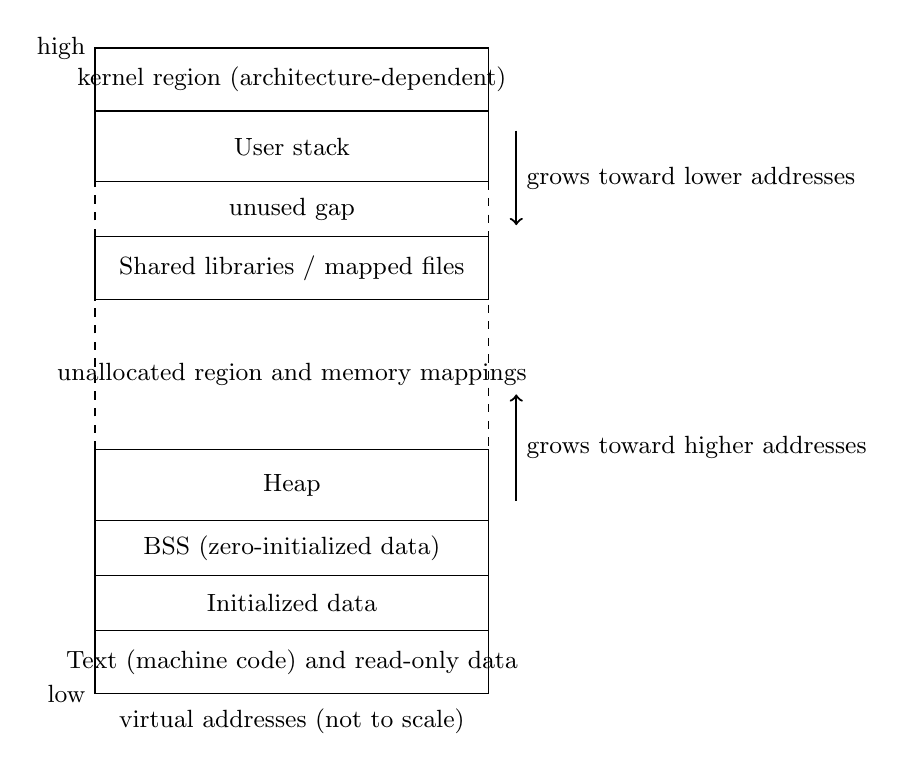
\begin{tikzpicture}[font=\small]
  \draw (0,0) rectangle (5,0.8);
  \node at (2.5,0.4) {Text (machine code) and read-only data};
  \draw (0,0.8) rectangle (5,1.5);
  \node at (2.5,1.15) {Initialized data};
  \draw (0,1.5) rectangle (5,2.2);
  \node at (2.5,1.85) {BSS (zero-initialized data)};
  \draw (0,2.2) rectangle (5,3.1);
  \node at (2.5,2.65) {Heap};
  \draw[->,thick] (5.35,2.45) -- (5.35,3.8)
      node[midway,right] {grows toward higher addresses};
  \draw[dashed] (0,3.1) rectangle (5,5.0);
  \node[align=center] at (2.5,4.05)
      {unallocated region and memory mappings};
  \draw (0,5.0) rectangle (5,5.8);
  \node at (2.5,5.4) {Shared libraries / mapped files};
  \draw[dashed] (0,5.8) rectangle (5,6.5);
  \node at (2.5,6.15) {unused gap};
  \draw (0,6.5) rectangle (5,7.4);
  \node at (2.5,6.95) {User stack};
  \draw[->,thick] (5.35,7.15) -- (5.35,5.95)
      node[midway,right] {grows toward lower addresses};
  \draw (0,7.4) rectangle (5,8.2);
  \node[align=center] at (2.5,7.8)
      {kernel region (architecture-dependent)};
  \node[left] at (0,0) {low};
  \node[left] at (0,8.2) {high};
  \node at (2.5,-0.35) {virtual addresses (not to scale)};
\end{tikzpicture}
\end{center}

\begin{itemize}
  \item \textbf{Text/code and read-only data:} This contains executable
  machine instructions and constants such as string literals.  It is
  normally readable and executable but not writable.  Because it is not
  modified, clean pages can be discarded and reloaded from the executable,
  and the same physical pages can be shared by several processes running the
  same program.

  \item \textbf{Initialized data:} Writable global and \texttt{static}
  variables having explicit nonzero initial values are stored here.  Their
  initial bytes are present in the executable file; for example,
  \texttt{static int count = 3;}.

  \item \textbf{BSS:} Writable global and \texttt{static} variables without
  an explicit initializer, or initialized to zero, belong here.  The
  executable records the required size rather than storing all the zero
  bytes; the loader supplies zero-filled memory.  For example,
  \texttt{static int table[1000];} is placed in BSS.

  \item \textbf{Heap:} This is the dynamically allocated region used by
  \texttt{malloc()} and related allocation routines.  Traditionally it
  begins after BSS and expands toward higher addresses via
  \texttt{brk}/\texttt{sbrk}; modern allocators also obtain separate
  mappings with \texttt{mmap}, particularly for large allocations.

  \item \textbf{Memory-mapping area:} Shared libraries, mapped executable
  objects, files mapped by \texttt{mmap}, and anonymous mappings are commonly
  placed between the heap and stack.  Shared library code pages may be
  physically shared while each process retains private writable state.

  \item \textbf{Stack:} The initial stack contains command-line arguments,
  the environment, and auxiliary-vector entries.  During execution it holds
  call frames, including return addresses, saved registers, parameters, and
  automatic local variables.  It conventionally grows toward lower
  addresses and is extended on demand up to a configured limit.

  \item \textbf{Kernel region:} Some architectures reserve a high part of
  the virtual address space for kernel mappings.  User-mode code cannot
  access these pages because page-table protection bits require kernel
  privilege.  On systems using kernel page-table isolation, most kernel
  mappings are absent while user code executes, but the protection principle
  is unchanged.
\end{itemize}

The address space also contains guard pages, for example below the stack, so
that an excessive growth causes a fault rather than silently corrupting
another region.  Thus, although the process appears to own one contiguous
address space, the valid regions have different permissions and need not be
contiguous in physical memory.

\subsection{Question 2: Disk I/O and running another process}
\begin{quote}
\itshape
Explain how a disk I/O request might allow the operating system to run
another process.
\end{quote}

\textbf{Solution.}
Consider process \(P_1\) executing a blocking \texttt{read()} whose requested
block is not in the page or buffer cache.

\begin{enumerate}
  \item \(P_1\) enters the kernel through a system call.  The kernel validates
  the request, creates or queues an I/O request for the disk controller, and
  arranges the destination buffer.  A controller may transfer the data by
  DMA, so the CPU need not copy each byte while the disk is operating.

  \item Because the read cannot yet return, the kernel changes \(P_1\)'s
  state from \emph{running} to \emph{waiting/blocked} on that I/O event.
  A blocked process is not eligible to use the processor.

  \item The scheduler chooses another process \(P_2\) from the ready queue.
  The OS performs a context switch: it saves \(P_1\)'s CPU state in its
  process control block (PCB), restores \(P_2\)'s saved registers and address
  space, and resumes \(P_2\).  Computation by \(P_2\) therefore overlaps the
  comparatively slow disk operation.  If no process is ready, the CPU
  executes the idle task instead.

  \item When the disk operation completes, the controller raises an
  interrupt.  The interrupt handler records completion, and the kernel wakes
  \(P_1\), moving it from the waiting queue to the ready queue.  The
  scheduler may run it immediately or later according to the scheduling
  policy.  When \(P_1\) next runs, the system call returns the data or an
  error status.
\end{enumerate}

Thus blocking I/O blocks the requesting process, not the entire processor.
The OS uses multiprogramming to keep the CPU useful during the I/O latency.
With asynchronous or nonblocking I/O, the caller itself need not block, but
the same interrupt-driven completion mechanism is normally used.

\subsection{Question 3: Creation of a new process}
\begin{quote}
\itshape
Illustrate the steps performed by an OS to create a new process.  What common
events lead to the creation of a process?
\end{quote}

\textbf{Solution.}
A process is an executing program together with an address space, CPU
context, kernel-maintained resources, and scheduling state.  A typical OS
performs the following steps:

\begin{enumerate}
  \item \textbf{Create kernel bookkeeping.} Allocate a unique process ID and
  a PCB (or task structure).  Initialize parent/child links, credentials,
  accounting data, signal state, resource limits, and the initial process
  state.

  \item \textbf{Create an address space.} Allocate page-table structures and
  virtual regions for code, data, BSS, heap, mappings, and stack.  In a
  Unix-like \texttt{fork()}, the child initially receives a logical copy of
  the parent's address space; copy-on-write allows parent and child to share
  physical pages until either writes.  When loading a new executable, as in
  \texttt{exec()}, the loader instead maps the executable's segments,
  zero-fills BSS, maps required shared libraries, and builds a fresh user
  stack containing \texttt{argv}, the environment, and auxiliary data.

  \item \textbf{Set up execution context.} Allocate a kernel stack and
  construct the saved register/trap-frame state.  Set the initial program
  counter, user stack pointer, processor mode, and other architecture state
  so that dispatch begins at the correct entry point.  After
  \texttt{fork()}, parent and child resume after the same call, but
  \texttt{fork()} returns the child's PID in the parent and \(0\) in the
  child.

  \item \textbf{Set up resources.} Establish the process's current directory,
  root directory, open-file descriptor table, terminal, signal dispositions,
  and IPC state.  A child commonly inherits references to many of these
  resources from its parent; the references, not necessarily the underlying
  objects, are copied.

  \item \textbf{Admit it for execution.} Apply admission and security checks,
  mark the process \emph{ready}, and insert it into an appropriate scheduler
  ready queue.  On a later dispatch, the scheduler restores its context and
  it begins or resumes user-mode execution.
\end{enumerate}

Unix commonly separates creation and program loading: a shell calls
\texttt{fork()} to create a child, the child calls an \texttt{exec} function
to replace its image, and the parent may call \texttt{wait()} for completion.
Other systems provide a combined \emph{spawn} operation.

Common events that cause process creation include:
\begin{itemize}
  \item \textbf{System initialization:} During boot, the kernel starts the
  initial user process, which starts services and daemons.
  \item \textbf{Interactive login or command execution:} A login service
  creates a user session and shell; the shell forks/spawns a process for a
  command or pipeline stage.
  \item \textbf{An explicit request by an existing process:} A program calls
  \texttt{fork()}, \texttt{posix\_spawn()}, or an equivalent creation API,
  for example to perform work concurrently.
  \item \textbf{Batch-job submission:} A batch scheduler admits a submitted
  job and starts one or more processes when resources become available.
  \item \textbf{A user or service request:} A server may create a worker
  process to handle a connection, print request, compilation, or other
  service operation.  Process pools are often used instead, in which case
  workers are created in advance.
\end{itemize}

\subsection{Question 4: Interleaved execution of three processes}
\begin{quote}
\itshape
Show the traces of three processes and illustrate interleaved execution
(with instruction cycles, I/O, context switch, etc.) of these processes
performed by the processor.
\end{quote}

\textbf{Solution.}
Consider three processes that are all ready at time \(0\).  Their individual
traces are
\[
\begin{array}{c@{\quad:\quad}l}
P_1 & \mathrm{CPU}(3),\ \mathrm{I/O}(4),\ \mathrm{CPU}(2),\ \mathrm{exit},\\
P_2 & \mathrm{CPU}(2),\ \mathrm{I/O}(3),\ \mathrm{CPU}(3),\ \mathrm{exit},\\
P_3 & \mathrm{CPU}(4),\ \mathrm{exit}.
\end{array}
\]
Numbers denote time units.  Assume FCFS selection of ready processes,
nonpreemptive CPU bursts, one time unit for each context switch, and that I/O
devices operate concurrently with the CPU.  One possible complete execution
is:

\begin{center}
\small
\begin{tabular}{c|l|l|l|l}
\textbf{Time} & \textbf{Processor} & \(\boldsymbol{P_1}\) &
  \(\boldsymbol{P_2}\) & \(\boldsymbol{P_3}\)\\ \hline
\(0\)--\(3\)   & execute \(P_1\) CPU burst & running & ready & ready\\
\(3\)--\(4\)   & context switch \(P_1\!\to\!P_2\) &
  blocked (I/O \(3\)--\(7\)) & selected & ready\\
\(4\)--\(6\)   & execute \(P_2\) CPU burst &
  blocked & running & ready\\
\(6\)--\(7\)   & context switch \(P_2\!\to\!P_3\) &
  blocked & blocked (I/O \(6\)--\(9\)) & selected\\
\(7\)--\(9\)   & execute \(P_3\) & ready & blocked & running\\
\(9\)--\(11\)  & execute \(P_3\) & ready & ready & running\\
\(11\)--\(12\) & context switch \(P_3\!\to\!P_1\) &
  selected & ready & terminated\\
\(12\)--\(14\) & execute \(P_1\) CPU burst &
  running & ready & terminated\\
\(14\)--\(15\) & context switch \(P_1\!\to\!P_2\) &
  terminated & selected & terminated\\
\(15\)--\(18\) & execute \(P_2\) CPU burst &
  terminated & running & terminated
\end{tabular}
\end{center}

Equivalently, the processor timeline is
\[
\underbrace{P_1}_{0\text{--}3}\;|\;
\underbrace{\mathrm{CS}}_{3\text{--}4}\;|\;
\underbrace{P_2}_{4\text{--}6}\;|\;
\underbrace{\mathrm{CS}}_{6\text{--}7}\;|\;
\underbrace{P_3}_{7\text{--}11}\;|\;
\underbrace{\mathrm{CS}}_{11\text{--}12}\;|\;
\underbrace{P_1}_{12\text{--}14}\;|\;
\underbrace{\mathrm{CS}}_{14\text{--}15}\;|\;
\underbrace{P_2}_{15\text{--}18}.
\]

Within each CPU interval, the processor repeatedly performs instruction
cycles: fetch an instruction using the current process's program counter,
decode it, execute it, and update architectural state.  At time \(3\),
\(P_1\)'s I/O instruction is realized through a system call; the OS starts
the device request and blocks \(P_1\).  During the context switch it saves
\(P_1\)'s registers, program counter, and stack pointer in its PCB and
restores those of \(P_2\).  I/O-completion interrupts at times \(7\) and \(9\)
move \(P_1\) and \(P_2\), respectively, back to the ready queue.  They resume
at the instruction following the blocking system call when later dispatched.
Thus each process observes its own sequential trace even though the single
processor interleaves their CPU bursts.  Timer preemption could produce a
finer interleaving; it is omitted here to keep the trace explicit.

\subsection{Question 5: C library wrapper and a Linux system call}
\begin{quote}
\itshape
Design a C program and show how a C library intercepts a function/statement
call along with invoking necessary system call in the Linux OS.
\end{quote}

\textbf{Solution.}
The following program writes a message to standard output using the POSIX
\texttt{write()} interface supplied by the C library.

\begin{lstlisting}[language=C]
#include <errno.h>
#include <stdio.h>
#include <unistd.h>

int main(void)
{
    const char msg[] = "Hello from user space\n";
    size_t done = 0;

    while (done < sizeof(msg) - 1) {
        ssize_t n = write(STDOUT_FILENO,
                          msg + done,
                          sizeof(msg) - 1 - done);
        if (n < 0) {
            if (errno == EINTR)
                continue;
            perror("write");
            return 1;
        }
        done += (size_t)n;
    }
    return 0;
}
\end{lstlisting}

The source-level \texttt{write()} is an ordinary user-space function call;
it is more precise to say that the C library \emph{wraps} the system call
than that it intercepts every C statement.  With dynamic linking, the call
is resolved through the executable's procedure linkage table/global offset
table to the \texttt{write} symbol in glibc.  The path is
\[
\boxed{\text{user \texttt{main}}}
\longrightarrow
\boxed{\text{glibc \texttt{write} wrapper}}
\longrightarrow
\boxed{\texttt{syscall} instruction}
\longrightarrow
\boxed{\text{Linux kernel system-call dispatcher}}
\longrightarrow
\boxed{\text{VFS/device implementation}}.
\]

On Linux for x86--64, the wrapper places the system-call number
\(\mathrm{SYS\_write}=1\) in register \texttt{rax} and the arguments
\(\texttt{fd}\), \(\texttt{buf}\), and \(\texttt{count}\) in
\texttt{rdi}, \texttt{rsi}, and \texttt{rdx}, respectively, then executes
the privileged-entry instruction \texttt{syscall}.  Other architectures use
different registers, numbers, and trap instructions.

The instruction changes control to a predefined kernel entry point and
changes privilege level; it does not create a new process.  The kernel saves
the user context, uses the system-call number to dispatch to the write
implementation, validates the file descriptor and user buffer, and sends the
request through the virtual file system to the object referenced by standard
output (for example, a terminal, pipe, or regular file).  It then returns a
result and restores user-mode execution.  A nonnegative return value is the
number of bytes accepted.  Linux kernel errors are represented internally
as negative error numbers; the glibc wrapper conventionally returns
\(-1\) and sets the thread-local variable \texttt{errno}.  The loop handles
interruption and partial writes.

For a higher-level call such as \texttt{printf()}, glibc first performs
formatting and user-space buffering.  It invokes a lower-level operation
such as \texttt{write()} only when the stream is flushed, so one
\texttt{printf()} statement does not necessarily correspond to one system
call.  The system-call boundary, not the ordinary library call itself, is
where controlled entry into the kernel occurs.
